\def\figpath{figures/flows/\valreg/}

% GP plots
\begin{figure}[hb]
    \centering
    \subfloat{ 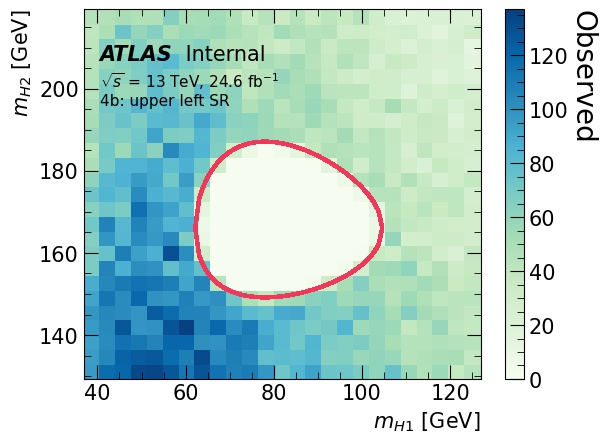
\includegraphics[width=0.22\textwidth]{\figpath/massplane_obs_16} }   
    \subfloat{ 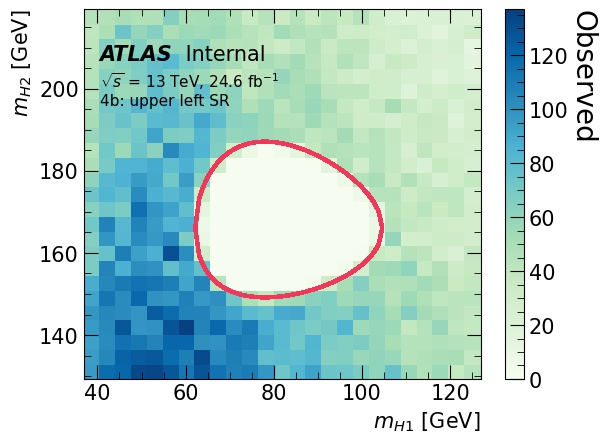
\includegraphics[width=0.22\textwidth]{\figpath/massplane_obs_16} }   
    \subfloat{ 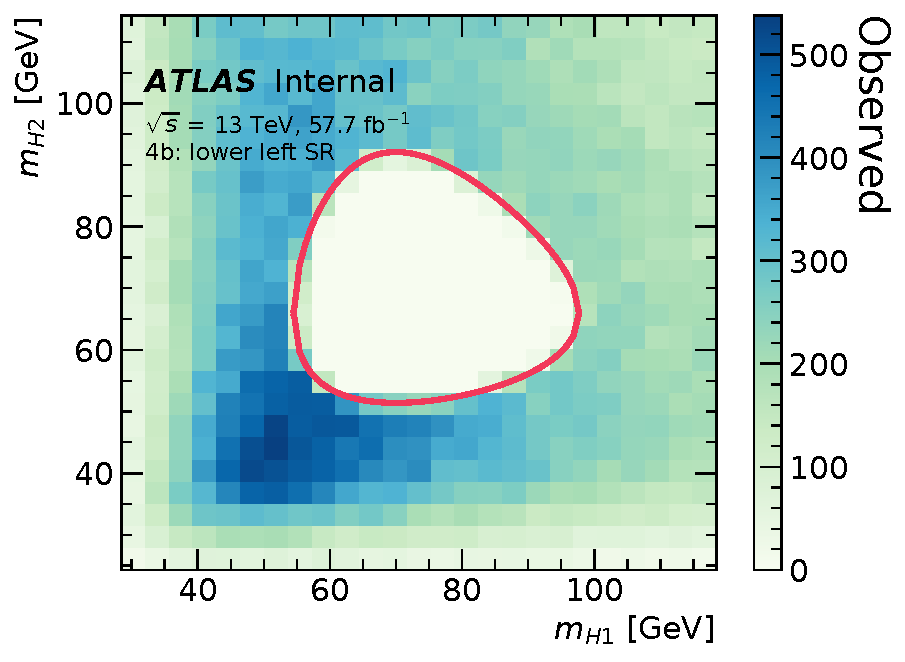
\includegraphics[width=0.22\textwidth]{\figpath/massplane_obs_18} }   
    \\
    \subfloat {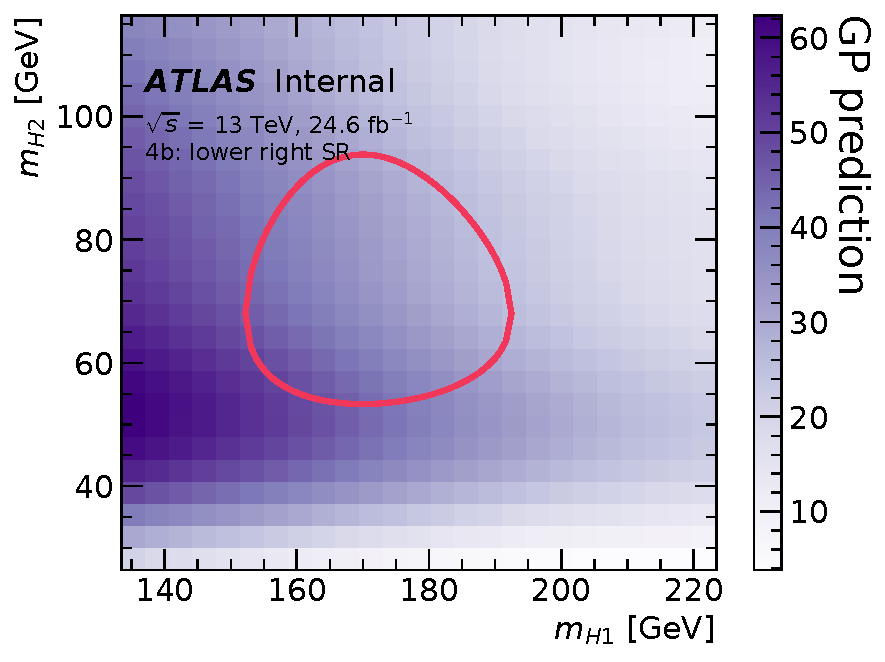
\includegraphics[width=0.22\textwidth]{\figpath/massplane_pred_16} }   
    \subfloat{ 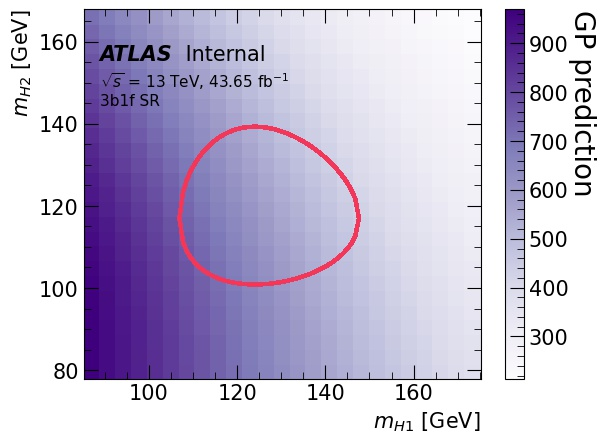
\includegraphics[width=0.22\textwidth]{\figpath/massplane_pred_17} }   
    \subfloat{ 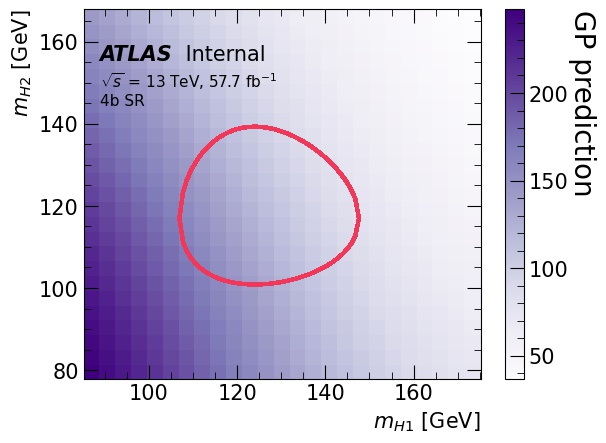
\includegraphics[width=0.22\textwidth]{\figpath/massplane_pred_18} }   
    \\
    \subfloat{ 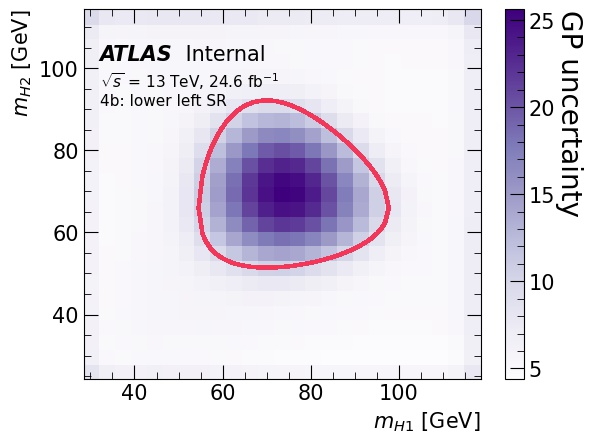
\includegraphics[width=0.22\textwidth]{\figpath/massplane_prederr_16} }   
    \subfloat{ 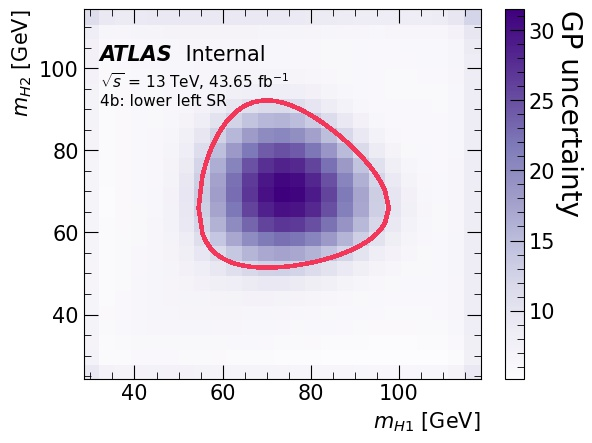
\includegraphics[width=0.22\textwidth]{\figpath/massplane_prederr_17} }   
    \subfloat{ 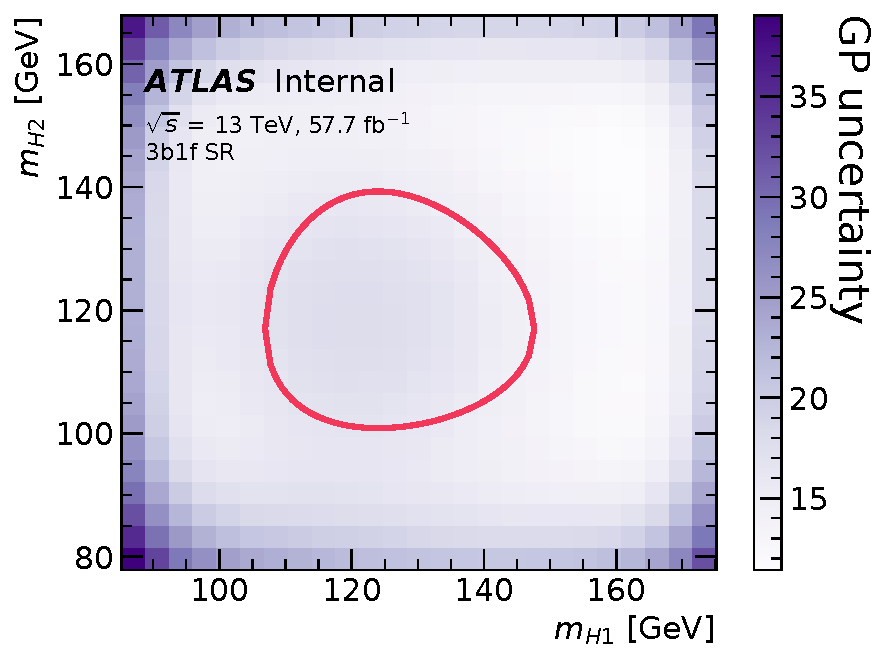
\includegraphics[width=0.22\textwidth]{\figpath/massplane_prederr_18} }   
    \\
    \subfloat{ 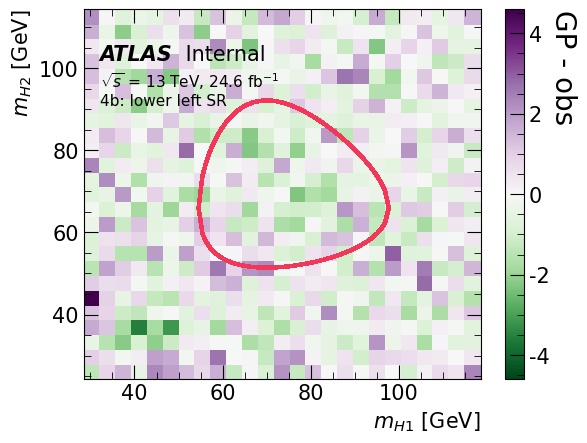
\includegraphics[width=0.22\textwidth]{\figpath/massplane_pred_minus_obs_over_sqrt_obs_16} }
    \subfloat{ 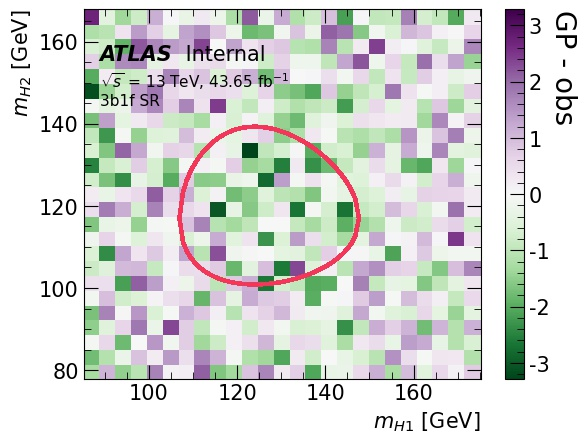
\includegraphics[width=0.22\textwidth]{\figpath/massplane_pred_minus_obs_over_sqrt_obs_17} }
    \subfloat{ 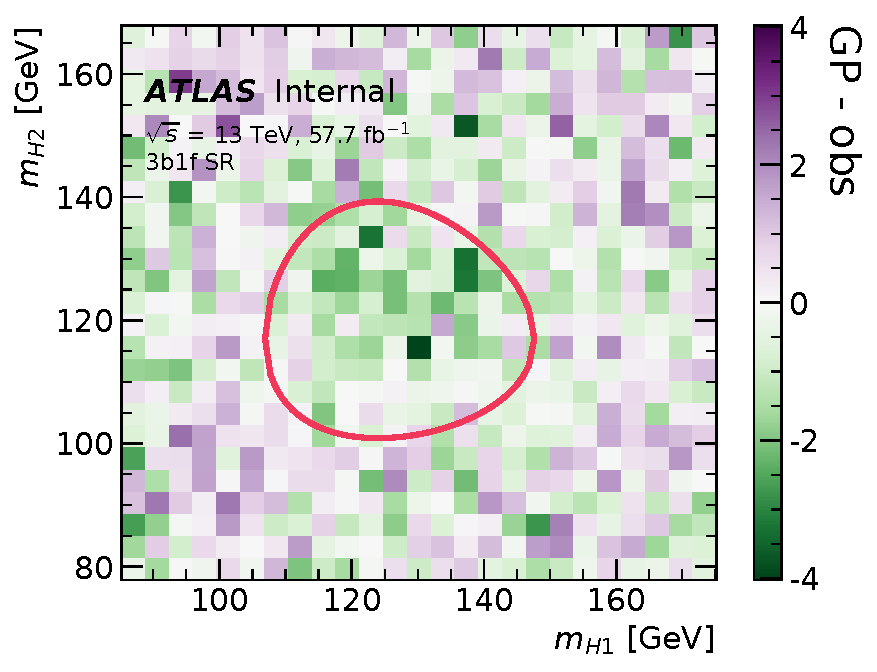
\includegraphics[width=0.22\textwidth]{\figpath/massplane_pred_minus_obs_over_sqrt_obs_18} }
    \\
    \subfloat{ 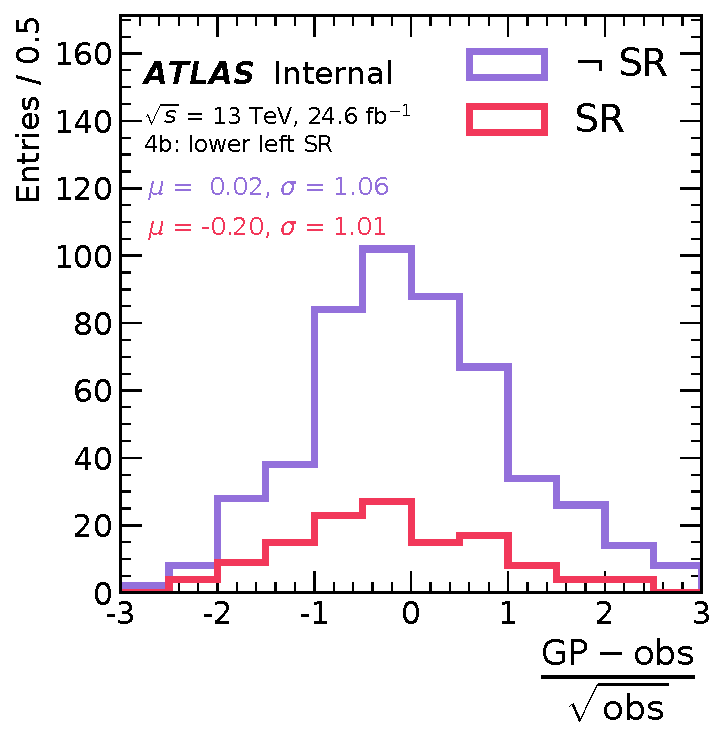
\includegraphics[width=0.18\textwidth]{\figpath/hist_pred_minus_obs_over_sqrt_obs_16}} \qquad
    \subfloat{ 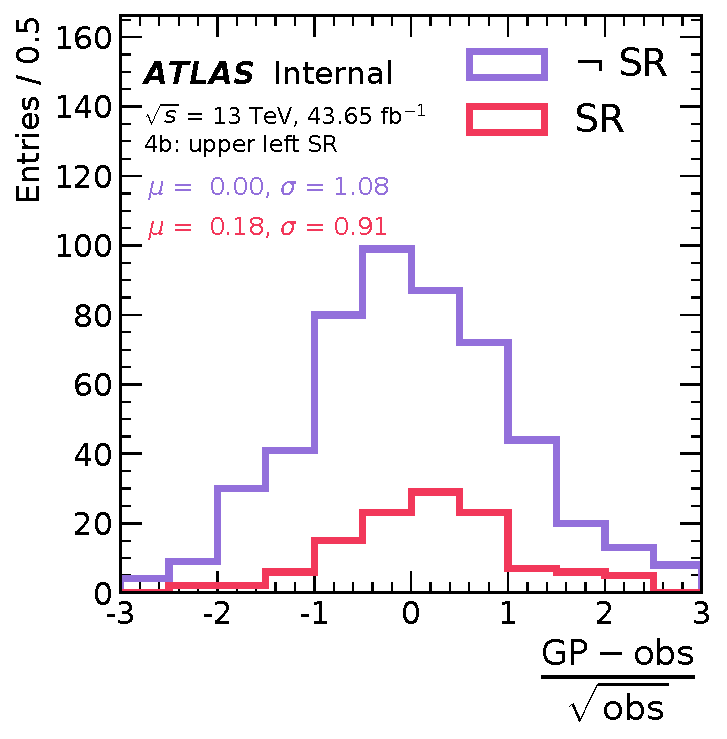
\includegraphics[width=0.18\textwidth]{\figpath/hist_pred_minus_obs_over_sqrt_obs_17}} \qquad
    \subfloat{ 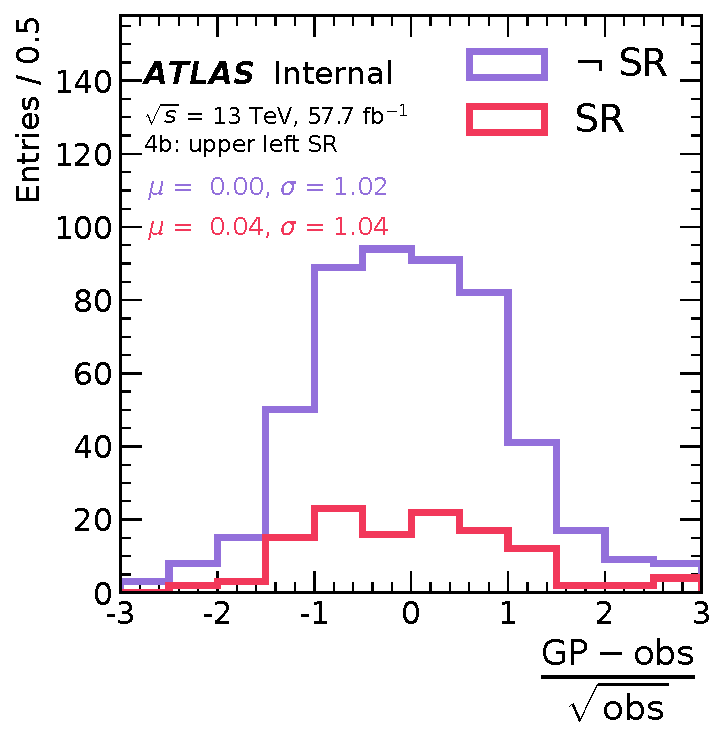
\includegraphics[width=0.18\textwidth]{\figpath/hist_pred_minus_obs_over_sqrt_obs_18}}
    \caption{GP fits for the \vallabel. All massplane fits are before the $X_{Wt}$ cut.}
    \label{fig:gp-\valreg}
\end{figure}

% The rest of the marginals
\begin{figure}[hbt]
    \centering
    \subfloat{ \includegraphics[width=0.3\textwidth]{\figpath/pT_h1_SR_Xwt_cut_rw_100_bs\baseTag.pdf} }
    \subfloat{ \includegraphics[width=0.3\textwidth]{\figpath/eta_h1_SR_Xwt_cut_rw_100_bs\baseTag.pdf} }
    \subfloat{ \includegraphics[width=0.3\textwidth]{\figpath/dphi_hh_SR_Xwt_cut_rw_100_bs\baseTag.pdf} }
    \\
    \subfloat{ \includegraphics[width=0.3\textwidth]{\figpath/pT_h2_SR_Xwt_cut_rw_100_bs\baseTag.pdf} }
    \subfloat{ \includegraphics[width=0.3\textwidth]{\figpath/eta_h2_SR_Xwt_cut_rw_100_bs\baseTag.pdf} }
    \subfloat{ \includegraphics[width=0.3\textwidth]{\figpath/X_wt_tag_SR_Xwt_cut_rw_100_bs\baseTag.pdf} }
    \\
    \subfloat{ \includegraphics[width=0.3\textwidth]{\figpath/m_hh_SR_Xwt_cut_rw_100_bs\baseTag.pdf} }
    \subfloat{ \includegraphics[width=0.3\textwidth]{\figpath/m_hh_cor2_SR_Xwt_cut_rw_100_bs\baseTag.pdf} }
    \subfloat{ \includegraphics[width=0.3\textwidth]{\figpath/dEta_hh_SR_Xwt_cut_rw_100_bs\baseTag.pdf} }
    \caption{Training and high level variables (post the $X_{Wt}$ cut) in the \vallabel validation region.}
    \label{fig:trainingvars-\valreg}
\end{figure}

\begin{figure}[hbt]
    \centering
    \subfloat{ \includegraphics[width=0.3\textwidth]{\figpath/pT_h1_SR_flow\baseTag.pdf} } 
    \subfloat{ \includegraphics[width=0.3\textwidth]{\figpath/eta_h1_SR_flow\baseTag.pdf} } 
    \subfloat{ \includegraphics[width=0.3\textwidth]{\figpath/dphi_hh_SR_flow\baseTag.pdf} } 
    \\
    \subfloat{ \includegraphics[width=0.3\textwidth]{\figpath/pT_h2_SR_flow\baseTag.pdf} }
    \subfloat{ \includegraphics[width=0.3\textwidth]{\figpath/eta_h2_SR_flow\baseTag.pdf} }
    \subfloat{ \includegraphics[width=0.3\textwidth]{\figpath/X_wt_tag_SR_flow\baseTag.pdf} }
    \\
    \subfloat{ \includegraphics[width=0.3\textwidth]{\figpath/m_hh_SR_flow\baseTag.pdf} }
    %\subfloat{ 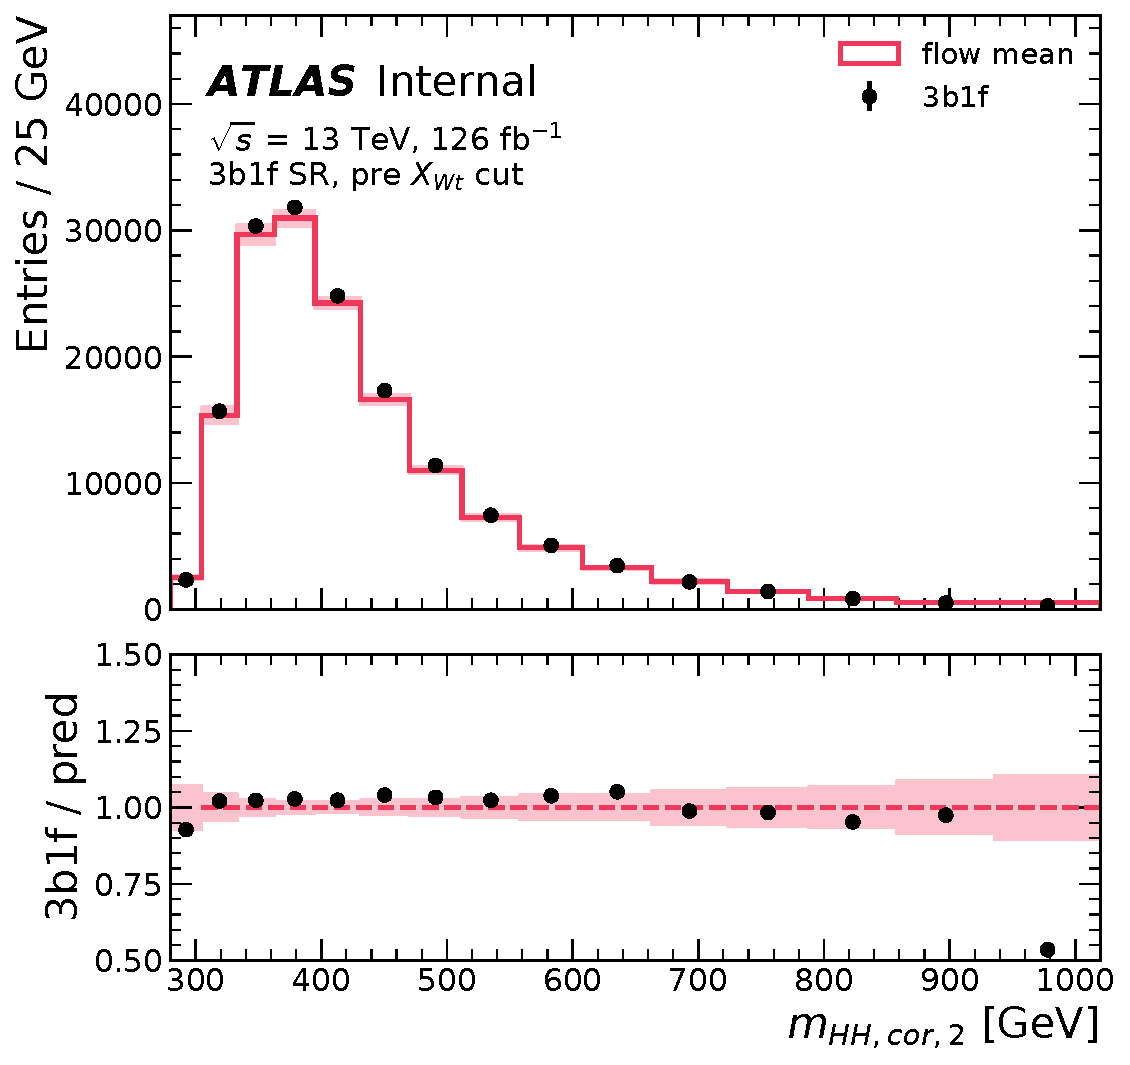
\includegraphics[width=0.3\textwidth]{\figpath/m_hh_cor2_SR_flow.pdf} }
    \subfloat{ \includegraphics[width=0.3\textwidth]{\figpath/dEta_hh_SR_flow\baseTag.pdf} }
    \subfloat{ \includegraphics[width=0.3\textwidth]{\figpath/pt_hh_SR_flow\baseTag.pdf} }
    \caption{Training variables (before applying the $X_{Wt}$ cut) in the \vallabel validation region.} 
    \label{fig:trainingvars-pre-Xwt-\valreg}
\end{figure}



% The high level discriminant plots
\begin{figure}[hbt]
    \centering
    \subfloat[After the $X_{Wt}$ cut]{ \includegraphics[width=\textwidth]{\figpath/X_hh_dEta_hh_m_hh_SR_Xwt_cut_rw_100_bs\baseTag.pdf} } \\
    \subfloat[Before the $X_{Wt}$ cut]{ \includegraphics[width=\textwidth]{\figpath/X_hh_dEta_hh_m_hh_SR_flow\baseTag.pdf} }
    \caption{High dimensional discriminant in the \vallabel validation region.}
    \label{fig:ggF-discs-\valreg}
\end{figure}
